\subsection{Izbira zobnikov in jermenov}
\subsubsection{Vrtilna hitrost glavnega vretena}
Na stroju imamo motor z vrtilno hitrostjo 1410 \( \frac{vrt}{min} \)
Po tabeli \nameref{tabela_za_izbiro_hitrosti} lahko razberemo, da potrebujemo jermen na motorju
\( d_1 = \phi 107 \) in \( d_2 = \phi 191 \).
Na spodnji sliki \ref{slika_prenosov} pa lahko vidimo shemo
zobniških in jermenskih prenosov.

\begin{figure}[H]
	\begin{center}
		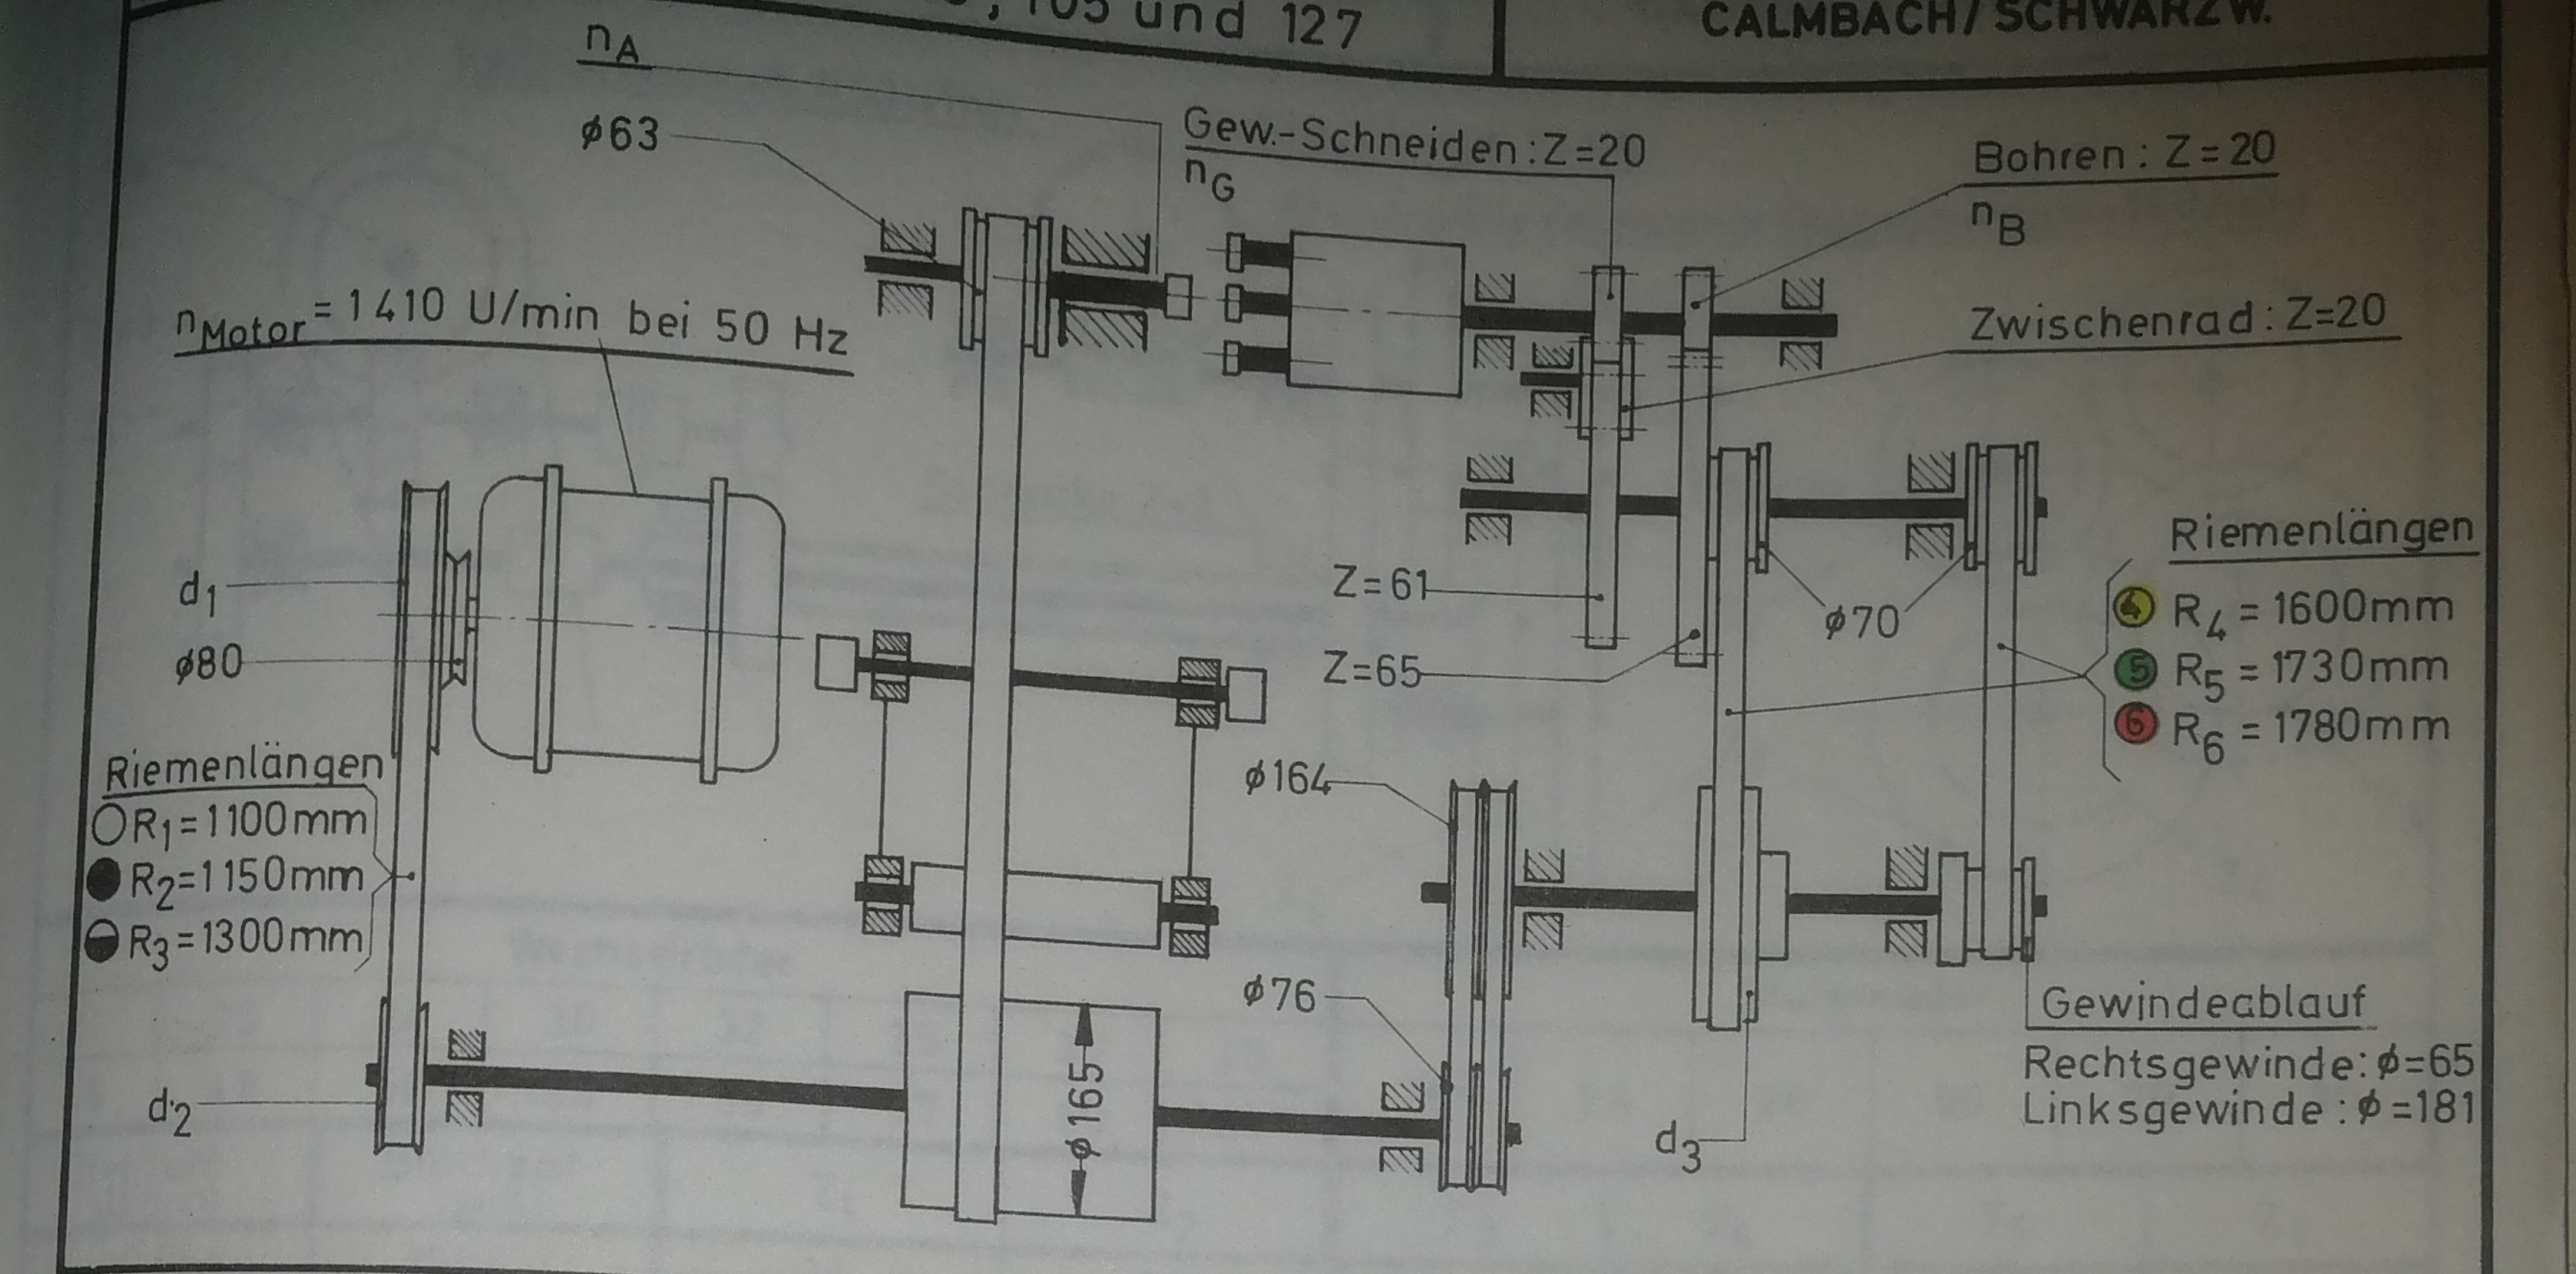
\includegraphics[width=\linewidth]{shema_prenosov_original.jpg}
		\caption{Slika sheme prenosov vrtilnih hitrosti
			\cite{gauthier}}
		\label{slika_prenosov}
	\end{center}
\end{figure}

Za boljšo preglednost sem zgornjo sliko \ref{slika_prenosov}
prerisal in jo prikazal na spodnji sliki \ref{skica_prenosov}

\begin{figure}[H]
	\begin{center}
		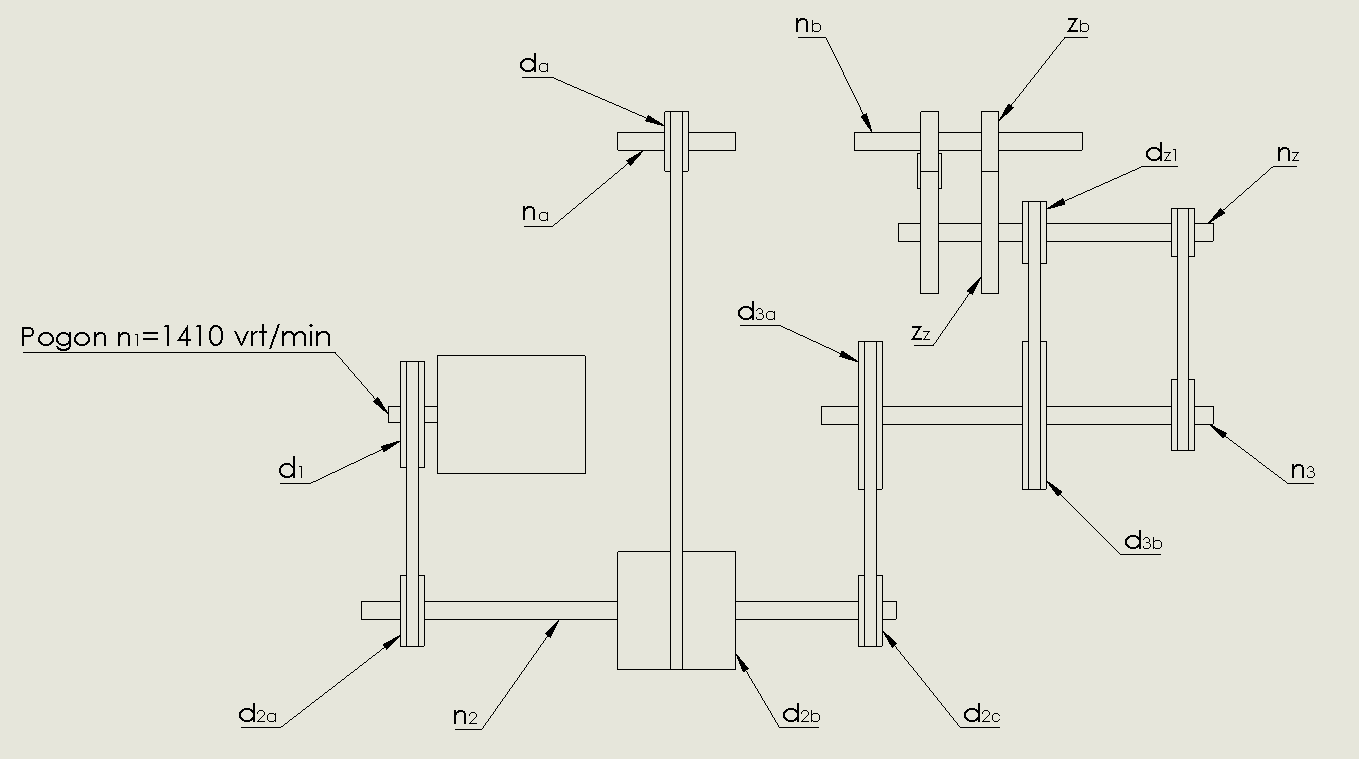
\includegraphics[width=\linewidth]{shema_prenosov_narisano.png}
		\caption{Prerisana shema prenosov vrtilnih hitrosti
			\cite{lasten}}
		\label{skica_prenosov}
	\end{center}
\end{figure}

Sedaj lahko izračunamo, če nam ta izbira res znese željeno hitrost glavnega vretena:
Prvo izračunamo razmerje med \( d_1 \) in \( d_2 \) in vrtilno hitrost osi \(n_2\)

\begin{equation}
	\label{eq:8}
	\begin{split}
		\frac{d_1}{d_2a} &= \frac{n_1}{n_2} \\
		n_2 &= \frac{d_2a}{d_1} * n_1 \\
		n_2 &= \frac{\phi 107}{\phi 191} * 1410 \frac{vrt}{min} = \\
		&= 789.95 \frac{vrt}{min} \approx 790 \frac{vrt}{min}
	\end{split}
\end{equation}

Ker so vrtljaji motorja redkokdaj točni, bom zaokrožil vrednost. Sedaj
lahko pa z njo izračunamo vrtljaje glavnega vretena, kot tudi jermene
potrebne za gnana orodja. Prvo bom preveril, če se glavno vreteno vrti z
pravilno hitrostjo

\begin{equation}
	\label{eq:9}
	\begin{split}
		\frac{d_2b}{d_a} &= \frac{n_2}{n_a} \\
		n_a &= \frac{d_a}{d_2} * n = \\
		n_a &= \frac{\phi 165}{\phi 63} * 790 \frac{vrt}{min} = 2069 \frac{vrt}{min}
	\end{split}
\end{equation}

Dobil sem malo večjo hitrost, kot sem želel, vendar je to praktično zanemarljivo.

\subsubsection{Vrtilna hitrost gnanih orodij}
Iz tabele \ref{tabela_operacij} razberemo da je željena hitrost 4200 \(\frac{vrt}{min}\).
Ker imamo na glavnem vretenu 2000 \(\frac{vrt}{min}\) potrebujemo na gnanih orodjih
še 2200 \(\frac{vrt}{min}\). Nato iz tabele \nameref{tabela_za_izbiro_hitrosti} v prilogi
razberemo da za to potrebujemo premer osi \(d_3 = \phi 143\). Za začetek moram
še izračunati obrate na osi \(n_3\)

\begin{equation}
	\label{eq:10}
	\begin{split}
		\frac{d_2c}{d_3a} &= \frac{n_2}{n_3} \\
		n_3 &= \frac{d_3a}{d_2c} * n_2 = \\
		n_3 &= \frac{\phi 164}{\phi 76} * 790 \phi \frac{vrt}{min} = 1705 \frac{vrt}{min}
	\end{split}
\end{equation}

Takšni so vrtljaji na gredi \(n_3\) ki nam omogoča da vrtamo ali pa vrezujemo navoje.
Izberemo tisti jermen, ki je za vrtanje, ki poganja zobniško gred \(n_z\), ki
poganja svedre \(n_b\). Jermen iz \(d_3b\) ni direktno vezan na gred svedrov,
ker se celotna konstrukcija skupaj z končno gredjo premika skupaj z
svedri. Zato so uporabljeni široki zobniki, kateri nam omogočajo to gibanje
v vzdolžni smeri in ne jermen. Zdaj še izračunam preostala razmerja

\begin{equation}
	\label{eq:11}
	\begin{split}
		n_z &= \frac{d_z}{d_3} * n_3 = \\
		n_z &= \frac{\phi 70}{\phi 143} * 1705 \frac{vrt}{min} = 835 \frac{vrt}{min}
	\end{split}
\end{equation}

Zobniška gred se vrti z hitrostjo \(835 \frac{vrt}{min}\). Zdaj pa zračunam
zadnji prenos iz nje na svedre. Ker je to zobniško razmerje bom namesto
premera uporabil število zobnikov kot tudi prestavno razmerje za zobnike

\begin{equation}
	\label{eq:12}
	\begin{split}
		\frac{z_b}{z_z} &= \frac{n_z}{b_b} \\
		n_b &= \frac{z_z}{z_b} * n_z = \\
		n_b &= \frac{65 zob}{20 zob} * 835 \frac{vrt}{min} = 2713 \frac{vrt}{min}
	\end{split}
\end{equation}

Izračunana vrtilna hitrost svedrov je veliko večja od pričakovane \(2000\frac{vrt}{min}\),
ampak nam bo to pri vrtanju tako majhne luknje še prav prišlo.

\subsubsection{Določitev zobnikov krivuljne gredi}

Iz tabele v \nameref{tabela_krivuljna_gred} razberemo željen čas
ali pa čim boljši približek. V našem premeru je to čas 10.21 s.
Spodaj na sliki \ref{povecava} je povečava slike iz \nameref{tabela_krivuljna_gred}
\begin{figure}[H]
	\begin{center}
		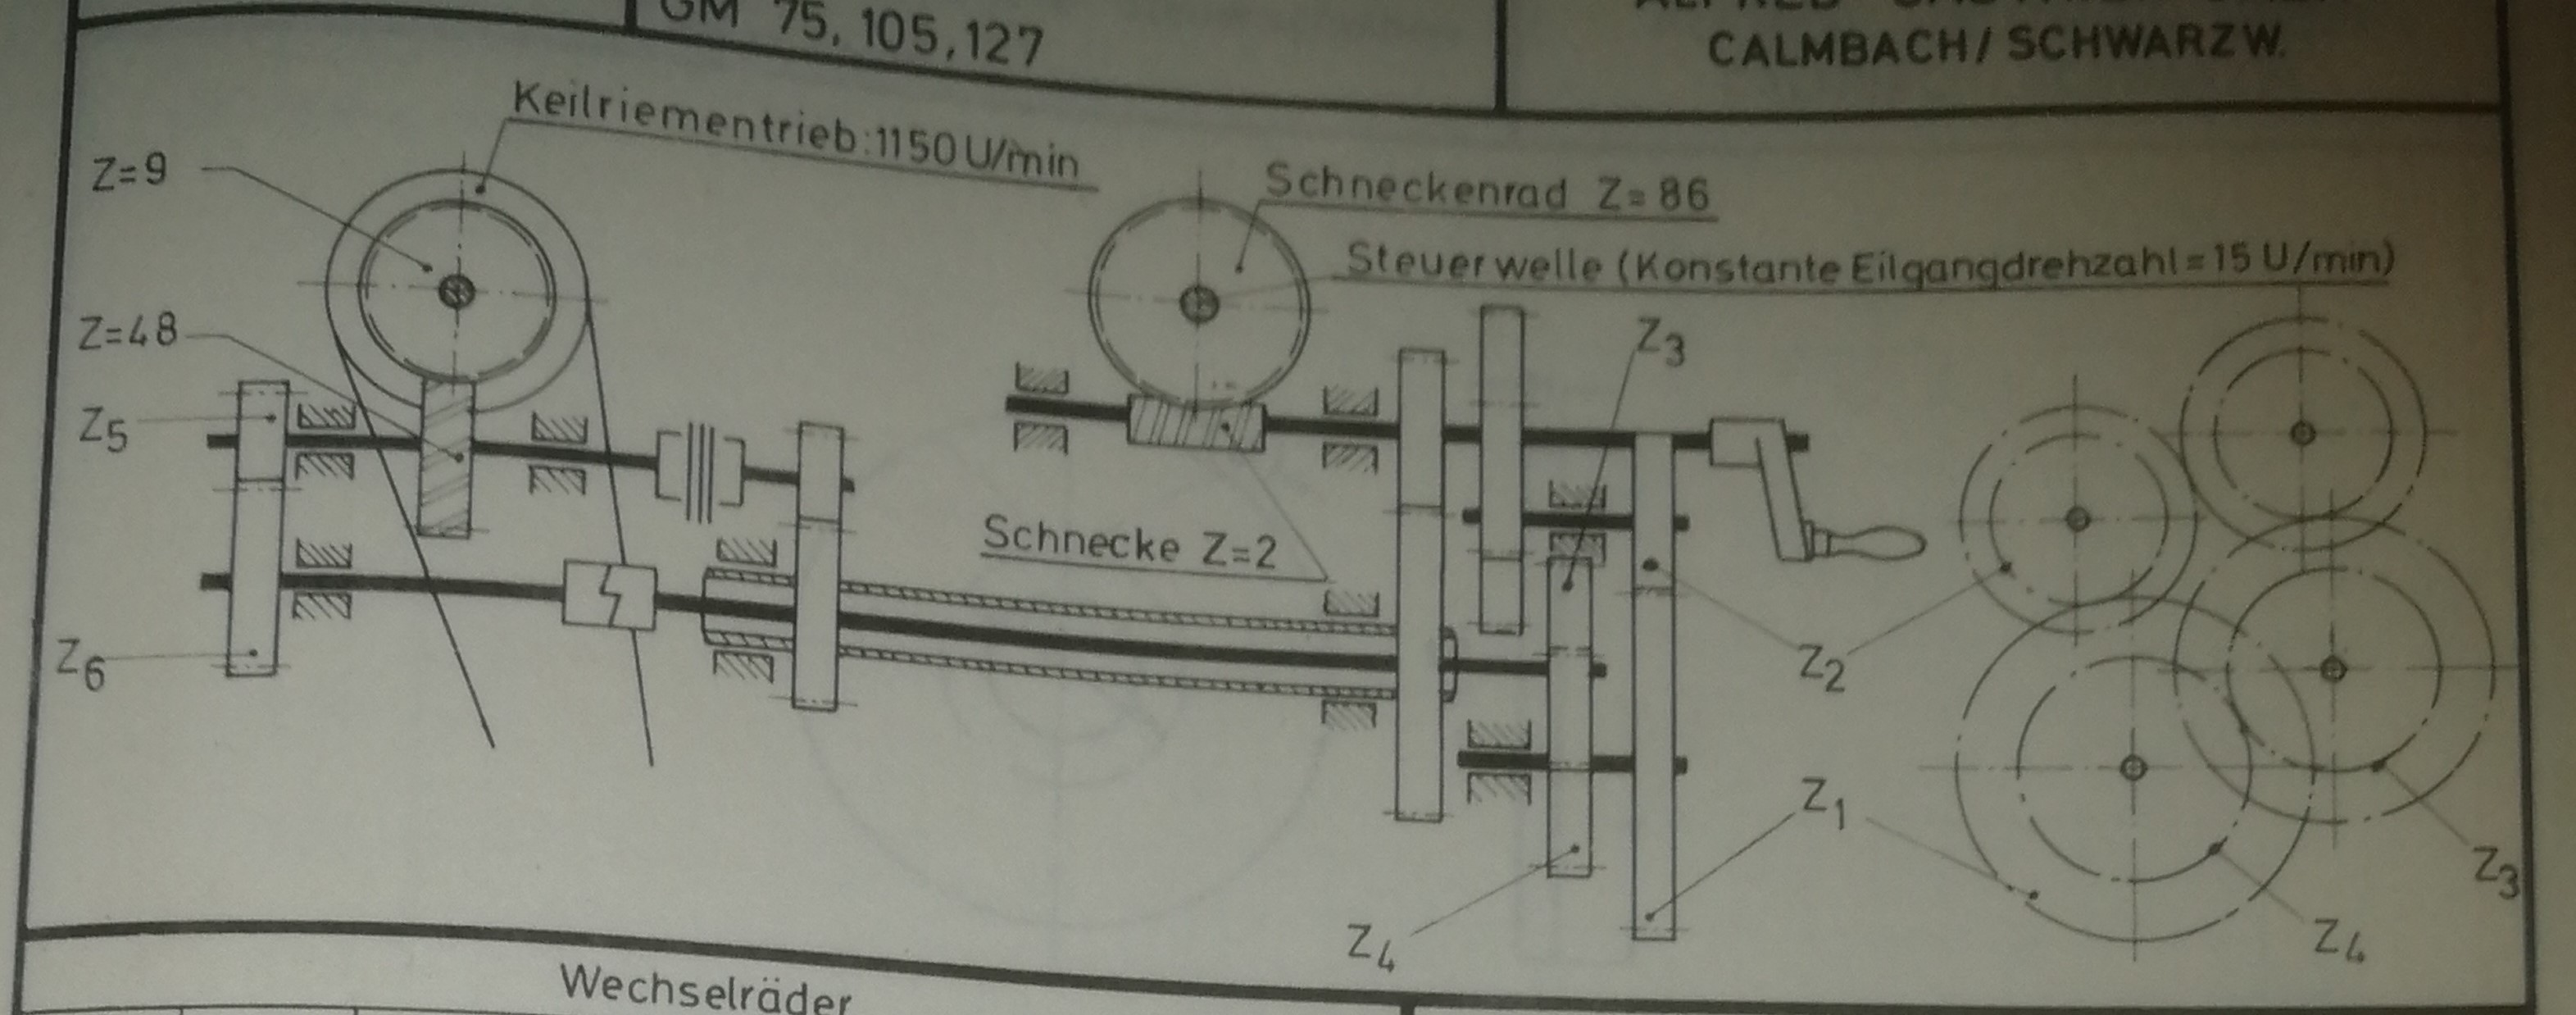
\includegraphics[width=\linewidth]{shema_tabela_krivuljna_gred.jpg}
		\caption{Povečava sheme jermenov in zobnikov
			hitrosti krivuljne gredi
			\cite{gauthier}}
		\label{povecava}
	\end{center}
\end{figure}

Potem še določimo vse potrebne zobnike tako, da jih razberemo iz tabele: \\
\(Z_1 = 45 zob, Z_2 = 40 zob, Z_3 = 25 zob, Z_4 = 60 zob, Z_5 = 70 zob, Z_6 = 26 zob\).
Ostali zobniki pa ostanejo enaki.

Zdaj ko imamo vse krivulje in zobnike preračunane, nam preostane še montiranje stročnic in orodja.